\documentclass[a4paper,12pt]{report}
\usepackage{color}
\usepackage{graphicx}
\usepackage{amssymb}
\usepackage{amsmath}
\usepackage{caption}
\usepackage{subcaption}
\begin{document}
\chapter{Absolute Stability: pictorial depiction}
\section{Methodology}
We define a region $R$ of absolute stability for a one step method as the region  in the complex plane satisfying :
\[R = {\lambda \Delta t \in C, |Q(\lambda \Delta t)|<1}\]
We are dealing here with methods which involve more than one evaluation steps. Range Kutta Methods are attributed to be multi stage methods. The other class of methods for which involve multi steps are known as the multi-step methods. The difference between the two is that in the case of Range Kutta methods, we evaluate intermediate values by taking small steps like a half step and proceed to next step ignoring the previous intermediate step informations. In the other case, the values from previous steps are not discarded but kept and used for reaching the higher order. The region of absolute stability \textbf{(ROS)} of the latter type having linearity can be evaluated by simply solving the equation $u^{\prime}(t)=\lambda u(t)$ using the method in question. An expression for amplification factor is thus obtained. A contour plotter has to be employed to border the area which has $|g| = 1$. \\
As we know the equation we are trying to solve here is a partial differential equation, hence there are two discretizations involved. The absolute stability analyis would be a little bit more involved. Perhaps we will also employ the Von-Neumann analysis to simplify the process of obtaining the stability criteria. However the absolute stability for the combination is slightly different from and is known as the method of lines. We would be following the procedure as mentioned by LeVeque R. L. in his book "Finite Difference Methods for Differential Equations". \\
We are using RK method and upwind or central difference schemes for time and space discretization respectively. The problem can thus be broken down in two segments such that the interaction between the two discretization is accounted for in one of the two parts. LeVeque has discribed the procedure for hyperbolic equations while using Central difference scheme to discretize the space coordinates and has tested many time discretization with it to determine the stability obtaining a group of equations having Euler type representation and using the Euler stability region to approximate that if it is possible that the eigen values of the given solution can ever yield a stable solution. We would be using the same procedure to graphically determine the stability but for different set of methods obviously (instead of Lax Wendroff method used by LeVeque). \\
Firstly the time discretization scheme has to be solved to determine the stability region corresponding to that scheme. Next we solve the the hyperbolic equation discretizing it in both the domains converting the equations into a system with a matrix representation similar to $U^{\prime}(t) = BU(t)$ where B is a scalar matrix and U(t) is a vector field. The obtained system will be used to obtain the eigen value of the system and then one can check it if it lies in the stability region (say $S$) obtained in the first step.
\section{ROS: Only RK method }
The corresponding expressions and eigen region of stability for the three Runge Kutta methods presently under discussion are being presented here.
\newline For \textbf{RK 2}, the expression evaluates as below:
\begin{eqnarray}
a&=&\Delta t f(v^n,t^m) \nonumber \\
b&=&\Delta t f(v^n+a/2,t^n+\Delta t/2) \nonumber \\
v^{n+1} &=& v^n+ b \nonumber
\end{eqnarray}
Using the scheme on $u^{\prime}(t)=\lambda u(t)$ and solving for u, we get
\[u^{n+1}=u^n+\lambda \Delta t (u^n+\frac{\lambda \Delta t u^n}{2})\]
\[\Rightarrow g(\lambda \Delta t)  = 1+\lambda \Delta t + \frac{(\lambda \Delta t)^2}{2}\]
\\ or $g(z)  = 1+z + \frac{z^2}{2}$ where z is a complex number. The gain so obtained after limiting with the bound of 1 has region located in the left side of the imaginary axis. Its a near elliptic surface symmetric with respect to x axis. 
\begin{figure}[h!]  
	\centering
	\begin{subfigure}[b]{0.4\textwidth}
		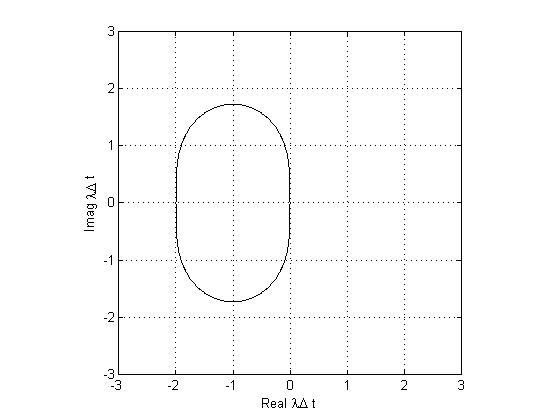
\includegraphics[width=\textwidth]{rk2.jpg}
                \caption{RK 2}
	\end{subfigure}
	\begin{subfigure}[b]{0.4\textwidth}
		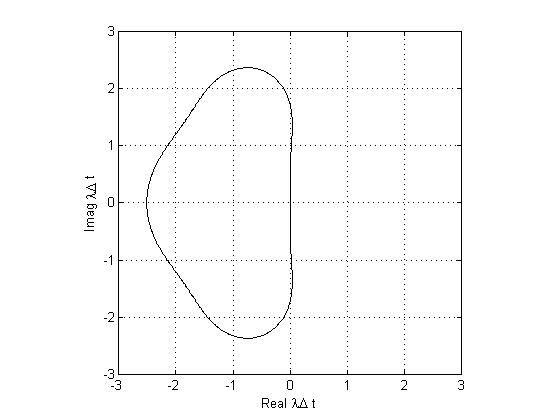
\includegraphics[width=\textwidth]{rk3.jpg}
                \caption{RK 3}
	\end{subfigure}
	\begin{subfigure}[b]{0.4\textwidth}
		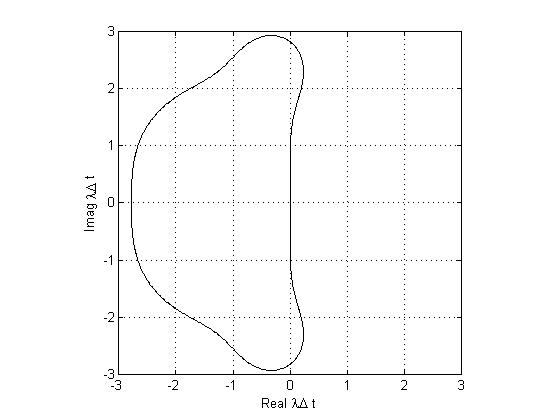
\includegraphics[width=\textwidth]{rk4.jpg}
                \caption{RK 4}
	\end{subfigure}
	\caption{Region of Stability for Range Kutta Method}
	\label{regofstab}
\end{figure}
Any differential equation which after discretization has the value of $\lambda \Delta t$ lying inside this bounded region would result in a stable solution using Runge Kutta Order 2 method. Moving ahead with \textbf{RK 3}, the amplification factor can be obtained as shown below
\begin{eqnarray}
y_{i+1} =& y_i + \frac{1}{6}h(k_1 + 4k_2 + k_3)
=& y_i + \frac{h}{6}(\lambda y_i +4\lambda(y_i+\frac{h\lambda y_i}{2})+\lambda (y_i -\lambda hy_j+2h\lambda(y_i+\frac{h\lambda y_i}{2}))) \nonumber \\
=& y_i + h\lambda y_i + \frac{(h\lambda)^2}{2} + \frac{(h\lambda)^3}{6} \nonumber \\
\Rightarrow =& g(z) = 1 + z + \frac{z^2}{2}+\frac{z^3}{6} \nonumber
\end{eqnarray}
while for \textbf{RK 4} the expressions can be similarly obtained to be as shown below:
\[ g(z) = 1 + z+ \frac{z^2}{2}+\frac{z^3}{6} + \frac{z^4}{24} \] 
Going through all the expressions one can easily see how with each order an extra term gets added which is basically expanding $u^{\prime}(t)$ and truncating the extension depending on the order of accuracy needed. This also verifies the basis of Runge Kutta methods. Region of eigen stability plots obtained are showcased in Figure \ref{regofstab}. Thus for an ODE to be solved using Runge Kutta methods, the value of $\lambda \Delta t$ should lie in the bounded regions which depends on the order of accuracy required.
\section{ROS: Both space \& time}
Now we already have the ROS for RK methods of all the requisite orders. Hence next we are trying to look how well does it work on the wave equation. We are now going to look into both the discretizations together. The wave equation has a first order differential operator for both space and time. Discretizing the space operator:
\[\frac{\partial u}{\partial t}= -a\frac{(u_{j+1}(t)-u_{j-1}()t)}{2h}\]
As we know the MOL needs a well defined cauchy problem with boundary conditions. So here we need the boundary conditions also. Using periodic boundary condition $u(0,t) = u(L,t)$, the problem becomes well posed and all the corresponding equations can now be written. Implementing the \textbf{RK 2} on the above equation and solving we get:
\begin{eqnarray}
u^{n+1}_{j}=&u^{n}_{j} -\frac{ak}{4h}(u^{*}_{j+1} -u^{*}_{j-1}) \nonumber \\
=& u^{n}_{j} - \frac{ak}{4h}u^{n}_{j+1}+(\frac{ak}{4h})^2(u^{n}_{j+2}-u^{n}_{j})+\frac{ak}{4h}-(\frac{ak}{4h})^2(u^{n}_{j}-u^{n}{j-2}) \nonumber \\
\end{eqnarray}
Converting this equation into differential form with $u^{\prime}_{j}(t)$ defined as that for Euler form $\frac{u^{n+1}_{j}-u^{n}_{j}}{k}$:
\[u^{\prime}_{j} = -\frac{a}{4h}(u^{n}_{j+1}-u^{n}_{j-1}) +k(\frac{a}{4h})^2(u^{n}_{j+2}+u^{n}_{j-2}-2u^{n}_{j})\]
All the corresponding equations including the boundary can be described as:
\begin{eqnarray}
u^{\prime}_{1} &=&  -\frac{a}{4h}(u^{n}_{2} - u^{n}_{m+1})+k(\frac{a}{4h})^2(u^{n}_{3}-2u^{n}_{1}+u^{n}_{m}) \nonumber \\
u^{\prime}_{2} &=&  -\frac{a}{4h}(u^{n}_{3} - u^{n}_{1})+k(\frac{a}{4h})^2(u^{n}_{4}-2u^{n}_{2}+u^{n}_{m+1}) \nonumber \\
for\ j\in[3,m-1] \nonumber \\
u^{\prime}_{j} &=& -\frac{a}{4h}(u^{n}_{j+1}-u^{n}_{j-1}) +k(\frac{a}{4h})^2(u^{n}_{j+2}+u^{n}_{j-2}-2u^{n}_{j}) \nonumber \\
u^{\prime}_{m} &=&  -\frac{a}{4h}(u^{n}_{m+1} - u^{n}_{m-1})+k(\frac{a}{4h})^2(u^{n}_{1}-2u^{n}_{m}+u^{n}_{m-2}) \nonumber \\
u^{\prime}_{m+1} &=&  -\frac{a}{4h}(u^{n}_{1} - u^{n}_{m})+k(\frac{a}{4h})^2(u^{n}_{2}-2u^{n}_{m+1}+u^{n}_{m-1}) \nonumber
\end{eqnarray}
This system of equations can be easily represented by the differential equation form given by:
$$\mathbf{U^{\prime}}(t) = \mathbf{AU}(t)$$ 
where 
\[ 
\mathbf{U}(t) = \begin{pmatrix}
u_{1}(t) \\ u_{2}(t) \\ \ldots \\ u_{m+1} \\
\end{pmatrix}
\ , \
\mathbf{U^{\prime}}(t) = \begin{pmatrix}
u^{\prime}_{1}(t) \\ u^{\prime}_{2}(t) \\ \ldots \\ u^{\prime}_{m+1} \\
\end{pmatrix}
\]
and
\[
\mathbf{A} = 
\frac{-a}{4h}
\begin{pmatrix}
0 & 1 & 0 & \ldots & 0 & -1 \\
-1& 0 & 1 & \ldots & 0 &  0 \\
0 & -1& 0 & \ldots & 0 &  0 \\
\vdots & \vdots & \vdots & \ddots & \vdots & \vdots \\ 
1 & 0 & 0 & \ldots & -1 & 0 \\
\end{pmatrix}
+\frac{a^2 k}{(4h)^2}
\begin{pmatrix}
-2& 0 & 1 & 0 & \ldots & 1 & 0 \\
0 &-2 & 0 & 1 & \ldots & 0 & 1 \\
1 & 0 &-2 & 0 & \ldots & 0 & 0 \\
\vdots & \vdots & \vdots & \vdots & \ddots & \vdots & \vdots \\
0 & 1 & 0 & 0 & \ldots & 0 & -2 \\
\end{pmatrix}
\]
Writing the two comprising matrix as $A_1$ and $A_2$
\[\mathbf{A} = \frac{-a}{4h} \mathbf{A_1} +\frac{a^2 k}{(4h)^2} \mathbf{A_2}\]
Since we have two matrices here, lets discuss them seperately. We are going to look into their properties which can help us estimate their eigen values since its their eigen values will help us determine the ROS.  \newline
\begin{itemize}
\item Matrix $A_1$ can be easily observed to be skew symmetric following the property $A_1^T = - A_1$. Now for a skew symmeteric matrix of order (m+1), there exist $\frac{(m+1)}{2}$ pairs of eigen values given $m+1$ is even or $\frac{m}{2}$ pairs and zero given $m+1$ is odd. The eigen values are also imaginary since all the elements of the matrix are real. The eigen values for this matrix are given by:
$$\beta_{p} = -2i \sin (2\pi ph),\ 	for\ p=1,\ 2,.....,m+1$$
\item Matrix $A_2$ is symmetric as it follows $A_2^T = A_2$. All the entries being real, this matrix has real eigen values. For m=4, the eigen values are $0, \pm3.618$ and $\pm1.382$, for m=5 the eigen values are 0 and -3 and for m=7, the eigen values are 0,-2 and -4. Let these values be $\alpha_i$.
\end{itemize}
Now the eigen values of the system can be written as:
$$\lambda_i = \alpha_i\frac{a^2}{(4h)^2}+i\frac{a}{2h}\sin(2\pi ph)$$
As the eigen values either lie on the left hand side of the argand plane and completely inside the region of Runge Kutta methods, hence these methods can be verified as \textbf{stable} for ak/2h < 1.\\
A similar analysis can also be done for the Upwind Scheme. In this case the evaluation of eigen values and 
\end{document}
